% 2008 年山东卷理科第 20 题：四棱锥 P-ABCD，底面 ABCD 为菱形，PA⊥平面 ABCD，
%   ∠ABC=60°，E、F 分别是 BC、PC 的中点。
% 来源 PDF：gaokaomath-src/普通高考/2008/2008山东理.pdf
% SHA-256：b4666951a0c2475fab098b837a343c7352003964f7811cedb1bdd610503e6e3b
% 原页：2008山东理.pdf 第 2 页（A3 三栏）第 1 栏，书页码 472。
% 重绘依据：按原页斜投影重绘：A 为被遮挡的后顶点，B 在左、C 在前、D 在右；
%   P—A、A—B、A—D、A—E 用虚线，E、F 分别为 BC、PC 的中点，E—F 虚线。
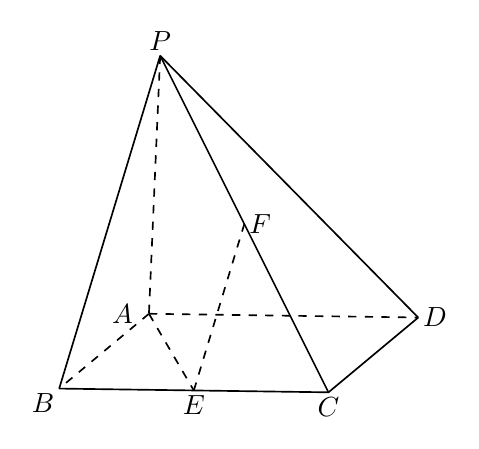
\begin{tikzpicture}[scale=0.95, semithick,
  every node/.style={inner sep=1.5pt}]

  \coordinate (A) at (2.20,1.50);
  \coordinate (B) at (1.00,0.50);
  \coordinate (C) at (4.60,0.45);
  \coordinate (D) at (5.80,1.45);
  \coordinate (P) at (2.35,4.95);
  \coordinate (E) at (2.80,0.475);
  \coordinate (F) at (3.475,2.70);

  % 可见棱
  \draw (P) -- (B);
  \draw (P) -- (C);
  \draw (P) -- (D);
  \draw (B) -- (C) -- (D);

  % 被遮挡的棱
  \draw[dashed] (P) -- (A);
  \draw[dashed] (A) -- (B);
  \draw[dashed] (A) -- (D);
  \draw[dashed] (A) -- (E);
  \draw[dashed] (E) -- (F);

  \node[above] at (P) {$P$};
  \node[left=4pt] at (A) {$A$};
  \node[below left] at (B) {$B$};
  \node[below] at (C) {$C$};
  \node[right] at (D) {$D$};
  \node[below] at (E) {$E$};
  \node[right] at (F) {$F$};
\end{tikzpicture}
